%%%%%%%%%%%%%%%%%%%%%%%%%%%%%%%%%%%%%%%%%%%%%%%%%%%%%%%%%%%%%%%%%%%%%%%%
\chapter{Algebraic Group Centrality Maximization for Large-Scale and
Disconnected Graphs}
\label{ch:ged-walk}
% Labels: approximate static, algebraic, sequential and parallel
%%%%%%%%%%%%%%%%%%%%%%%%%%%%%%%%%%%%%%%%%%%%%%%%%%%%%%%%%%%%%%%%%%%%%%%%
% ALENEX 2020

\section{Introduction}
%
As described in \Cref{ch:group-closeness-local-search,ch:group-harm-clos-max},
finding the most central group of vertices according to popular measures is a\change{n}
\np-hard problem. Since real-world applications may not require exact results,
approximation algorithms to maximize group centralities were introduced.
Despite a nearly-linear running time, algorithms for
group-betweenness~\cite{DBLP:conf/kdd/MahmoodyTU16,DBLP:conf/kdd/Yoshida14}
and, to a lesser extent, group-closeness~\cite{DBLP:conf/alenex/BergaminiGM18} and
group-harmonic (see \Cref{ch:group-harm-clos-max})
\change{fail to scale to large real-world instances due to high constant overheads}.

Moreover, a limitation of popular group centrality measures is that they are
based on shortest paths while some applications may be interested in all the
paths between two vertices (see \Cref{sec:prelim-resistance-distance}).
This motivated the introduction of electrical single-vertex centrality measures.
However, limited efforts were devoted to extend these measures to groups
of vertices. Only recently, Li \etal~\cite{DBLP:conf/www/0002PSYZ19}
proposed current flow group closeness centrality, \ie the extension
of electrical closeness to sets of vertices. As with electrical closeness,
this new group centrality measure -- without proper adjustments -- only
handles connected graphs, leaving the problem of electrical group centrality measures
for disconnected graphs open.

\paragraph{Contribution} In this chapter, we overcome the two aforementioned
limitations by introducing two new group centrality
measures: GED-Walk for \emph{group exponentially decaying walk} and group
forest closeness.

Inspired by
Katz centrality, GED-Walk takes into account walks of any length and considers
shorter ones \change{as} more important. We show our measure to be monotone and
submodular and we develop efficient nearly-linear parallel algorithms to
compute the GED-Walk score of a given group and to efficiently approximate the
group of $k$ vertices with highest GED-Walk centrality. Our greedy maximization
algorithm keeps lower and upper bounds of the marginal gain of every vertex to
the GED-Walk score and iteratively adds to the (initially empty) group the
vertex with highest marginal gain until the desired size is reached.

Group forest closeness, in turn, is the extension to groups of vertices
of forest closeness and, analogously, it handles disconnected graphs out of
the box.
To the best of our knowledge, we are the first to address the group case for this
centrality measure.
It turns out that group forest closeness centrality maximization is
\np-hard and we adapt the greedy approximation algorithm by Li
\etal~\cite{DBLP:conf/www/0002PSYZ19} to this problem.

Experiments show that our greedy algorithm for GED-Walk is two orders of
magnitude faster than the state of the art for group-betweenness
approximation~\cite{DBLP:conf/kdd/MahmoodyTU16}. Compared to the greedy
group-closeness heuristic~\cite{DBLP:conf/alenex/BergaminiGM18} and the greedy
approximation algorithm for group-harmonic (see \Cref{ch:group-harm-clos-max}),
we achieve a speedup of one to two orders of magnitude for groups with up to
100 vertices.
%
Further, for GED-Walk approximation, our
experiments indicate a running time that is in practice linear \wrt the input graph size
-- despite a higher worst-case time complexity.
We show potential applications for GED-Walk: (i) choosing a training set with high
GED-Walk score leads to improved performance for semi-supervised vertex classification
and (ii) features derived based on GED-Walk improve graph classification performance.

We repeat the semi-supervised vertex classification experiment on disconnected
graphs in order to demonstrate the practical usefulness of group forest closeness
as well.
Results demonstrate that our new measure improves upon existing measures as
well in the case of disconnected graphs.

\bibnotes{The contributions presented in this chapter about GED-Walk
were published in the Proceedings of the
\alenex{Twenty-Second}{2020} in collaboration with Alexander van der Grinten, Aleksandar
Bojchevski, Daniel Z{\"{u}}gner, Stephan G{\"{u}}nnemann, and Henning
Meyerhenke; the ones concerning group forest closeness
were published in the Proceedings of the \emph{Twenty-First SIAM International
Conference on Data Mining (SDM 2021)} in collaboration with
Alexander van der Grinten, Maria Predari, and
Henning Meyerhenke. About the former topic, the
development of the new measure GED-Walk and the implementation of the
algorithms for GED-Walk computation and maximization were a collaborative
effort of Alexander van der Grinten and
myself. Further, I \change{carried} out the experiments of
\Crefrange{sec:ged-walk:exp-scalability-k}{sec:ged-walk:impact-of-alpha}.
Regarding group forest closeness, my contributions involve the implementation of
the algorithm and carrying out the experiments.
Contributions not mentioned above are joint work with my coauthors. Proofs to which I
did not contribute are omitted and can be found in the original
papers~\cite{DBLP:conf/alenex/AngrimanGBZGM20,DBLP:conf/sdm/GrintenAPM21}.}

\paragraph{Related Work}
%
An overview of algorithms for maximizing established group centrality measures
is provided in \Cref{sec:lsh-gc-intro}.
The idea of developing alternative group centrality measures is not new. In fact, Ishakian
\etal~\cite{DBLP:conf/sdm/IshakianETB12} define single-vertex centrality measures based on
a generic concept of \emph{path} and generalize them to sets of vertices. In contrast
to GED-Walk, however, those measures are defined for directed acyclic graphs only.
Puzis \etal~\cite{puzis2007fast} introduce \emph{path betweenness centrality}, a group
centrality measure that counts the fraction of shortest paths that cross \emph{all}
vertices within the group.
Their proposed algorithms for finding groups with high path-betweenness are quadratic
in the best case (both in time and memory); hence, they cannot scale to large
networks -- indeed, the largest graphs considered in their paper have only 500 vertices.
Fushimi \etal~\cite{DBLP:conf/complexnetworks/FushimiSIK18} define a new
measure called \emph{connectedness centrality}, targeting the specific problem
of identifying the appropriate locations where to place evacuation facilities on
road networks. For this reason, their measure assumes the existence of edge failure
probabilities and thus it is not applicable to general graphs. Additionally,
due to expensive Monte Carlo simulations, computing their measure requires many
hours on graphs with \numprint{100000} edges, while GED-Walk handles graphs with
hundreds of millions of edges in minutes.

Finally, concerning electrical group centrality measures, Li
\etal~\cite{DBLP:conf/www/0002PSYZ19} defined current flow group closeness
centrality, \ie electrical closeness extended to set of vertices, and proposed
two greedy approximation algorithms to maximize this measure: (i) a
deterministic algorithm with $\Oh(n^3)$ running time and quadratic memory
requirements (it performs matrix inversions) and (ii) a faster randomized
algorithm with $\tilde{\Oh}(km\epsilon^{-2})$ running time ($\tilde{\Oh}$ hides
a polylogarithmic factor) that exploits JLT in combination with
\change{nearly linear time solvers for Laplacian and symmetric, diagonally
dominant, M-matrices.}

\section{Preliminaries}
\subsection{GED-Walk Centrality}
%
For GED-Walk, we deal with unweighted (possibly directed) graphs.
%
To avoid complexity-theoretic barriers typical of shortest-path based centrality
measures,\footnote{Recall from \Cref{ch:dyn-topk} (\Cref{sec:dyn-topk:intro})
that the existence
of a sub-cubic algorithm for betweenness (on general graphs) would also
imply the existence of a faster
algorithm for APSP~\cite{DBLP:conf/soda/AbboudGW15}. The vertex with
highest closeness, in turn, cannot be computed in sub-quadratic time unless
SETH~\cite{DBLP:journals/jcss/ImpagliazzoPZ01}
fails~\cite{DBLP:journals/im/BoldiV14} (see \Cref{ch:betweenness-approx},
\Cref{sec:betw-apx:betw-apx}).}
we derive our new measure from Katz centrality. As described in
\Cref{sec:centrality-measures},
Katz centrality is another popular centrality measure which can be computed more
efficiently compared to measures based on shortest paths.
Let $a_i(u) := \sum_{v \in V}\Adj^i[u, v]$ be the number of walks
of length $i$ that start at a vertex $u\in V$, where $\Adj$ is the adjacency
matrix of the graph.\footnote{Katz centrality is sometimes alternatively defined
by taking into account walks \emph{ending} at a given vertex; from an algorithmic
perspective, however, this difference is irrelevant.}
For a small enough attenuation $\alpha > 0$, the Katz
centrality of a vertex $u$ is defined as:

\begin{equation}
\label{eq:ged-walk:katz}
\katz(u) := \sum_{i = 1}^{\infty}\alpha^i \sum_{v \in V}\Adj^i[u, v] =
\sum_{i = 1}^{\infty}\alpha^i a_i(u),
\end{equation}

Note that $\katz(\cdot)$ does not
only consider \emph{shortest paths}, but \emph{walks} of any length -- with
shorter walks having higher importance due to the exponential decrease of
$\alpha^i$. Since it does not rely on APSP, $\katz(\cdot)$ can be computed faster
than betweenness centrality. For example, following from the algebraic formulation
of Katz centrality (see \Cref{eq:def:katz-alg}, \Cref{sec:centrality-measures}),
iterative linear solvers -- such as conjugate gradient -- can be used to
compute $\katz(\cdot)$ for all vertices at the same time.
Furthermore, efficient nearly-linear time algorithms for Katz centrality
approximation and ranking exist~\cite{DBLP:conf/esa/GrintenBGBM18}.
In fact, the algorithms that we present in this chapter are based on
those algorithms for Katz centrality.

In contrast to $\betw(\cdot)$ and $\clos(\cdot)$, however, replacing the single vertex
$u$ in \Cref{eq:ged-walk:katz} by a set leads to a rather uninteresting
measure: as $a_i(u)$ and $a_i(v)$ count distinct walks for $u \neq v$,
such a \enquote{group Katz} would just be equal to the sum of the individual
Katz scores. Hence, a group with maximal Katz centrality would just
consist of the top-$k$ vertices with highest $\katz(\cdot)$.
Indeed, this contrasts with the intuition of group centrality:
parts of a graph that are \emph{covered} by one vertex in the group
does \emph{not} need to be covered by a second group vertex.

Fortunately, we can construct a centrality measure satisfying this
intuition by replacing $\katz(\cdot)$ by a natural variant of it: instead of
considering all walks that \emph{start} at a given vertex $u$, we consider
all that \emph{cross} $u$. This leads to our definition
of ED-Walk:
%
\begin{definition}[ED-Walk]
Let $\phi_i(S)$ be the number of $i$-walks -- \ie walks of length $i$ -- that
contain at least one vertex in $S \subseteq V$. The ED-Walk (for \emph{Exponentially
Decaying} walk) centrality for $u \in V$ is:
%
\[
    \ed(u) := \sum_{i = i}^{\infty}\alpha^i \phi_i(\set{u}),
\]
%
where $\alpha > 0$ is a parameter of the centrality.
\end{definition}

As mentioned in \Cref{sec:centrality-measures}, in order for the series to
converge, $\alpha$ needs to be chosen small enough -- an upper limit for
$\alpha$ is provided in \Cref{sec:ged-walk:math-prop}.
As claimed above, ED-Walk naturally generalizes to a group measure:

\begin{definition}(GED-Walk)
The GED-Walk centrality of a group $S \subseteq V$ of vertices
is given by:
%
\begin{equation}
\label{eq:ged-walk:ged-walk}
\ged(S) := \sum_{i = 1}^{\infty}\alpha^i\phi_i(S).
\end{equation}
\end{definition}

In the context of group centrality, we are interested in two
problems:
\begin{itemize}
    \item the problem of computing the centrality of a \emph{given} group
        $S \subseteq V$;
    \item the problem of \emph{finding} a group that maximizes the
        group centrality measure.
\end{itemize}

We deal in particular with the latter optimization problem:

\begin{cproblem}{GED-Walk Maximization}
\begin{tabular}{ll}
\textbf{Input:} & Graph $G = (V, E)$, integer $1 \le k \le n$.\\
\textbf{Find:} & Set $S^\star \subset V$ with $|S| = k$ s.t. $\ged(S^\star)$ is maximum.
\end{tabular}
\end{cproblem}

Note again that, in contrast to Katz centrality, the GED-Walk maximization problem
is different from the top-$k$ ED-Walk centrality problem.


\subsection{Mathematical Properties of GED-Walk}
\label{sec:ged-walk:math-prop}
%
Since GED-Walk is based on similar concepts as Katz centrality, it is not surprising
that the two measures have analogous mathematical properties. Indeed,
the convergence properties of $\katz(u)$ and GED-Walk are
identical:

\begin{proposition}[\cite{DBLP:conf/alenex/AngrimanGBZGM20}]
\label{prop:ged-walk:convergence}
The following holds:
\begin{enumerate}
    \item $\ged(V) = \sum_{u \in V}\katz(u)$.
    \item Let $\sigma_{\max}$ be the largest singular value of the adjacency
        matrix of $G$. If $\alpha < 1 / \sigma_{\max}$, then $\ged(S)$ is
        finite for all $S \subseteq V$.
\end{enumerate}
\end{proposition}

Note that the quality of the first claim of \Cref{prop:ged-walk:convergence}
does not  hold for groups $S \subset V$.

We have now established that GED-Walk is a well-defined measure. In
the following, we prove further basic properties of the $\ged$ function:

\begin{proposition}
\label{prop:ged-walk:mon-submod}
GED-Walk is both non-decreasing and submodular as a set function.
\end{proposition}

\begin{proof}
Monotonicity is obvious from \Cref{eq:ged-walk:ged-walk}: as the input
set $S$ becomes larger, $\ged(S)$ cannot decrease. To see that
GED-Walk is also submodular, we observe that the marginal gain
$\ged(S \cup \set{u}) - \ged(S)$ is exactly the sum of the
number of walks that contain $u$ but no vertex in $S$, with
each walk weighted by a power of $\alpha$.
As such, the marginal gain can only decrease if $S$ is replaced
by a superset $T \supseteq S$.
\end{proof}

Given an algorithm to compute $\ged$, \Cref{prop:ged-walk:mon-submod}
would immediately allow us to construct a greedy algorithm to
approximate GED-Walk maximization -- as a consequence
\Cref{prop:prelim:greedy-apx}.
%
However, as we show in \Cref{sec:ged-walk:maximizing-ged}, we can
do better than naively applying the greedy approach.

As with other group centrality measures, maximizing GED-Walk turns
out to be an \np-hard problem~\cite[Theorem 2.1]{DBLP:conf/alenex/AngrimanGBZGM20}.

\section{Algorithms for GED-Walk}
\subsection{Computing GED-Walk Centrality}
\label{sec:ged-walk:compute-ged}
%
In this section, we address the problem of computing $\ged(S)$ of a given group
$S$. As we are not aware of an obvious translation of our $\ged(S)$ definition
to a closed form expression, we employ an approximation algorithm that computes
the infinite series of $\ged(S)$ up to an arbitrarily small additive constant
error $\epsilon > 0$.
%
To see how our algorithm works, let $\ell\in\natn$ be a positive integer.
We split the $\ged(S)$ series into the first $\ell$ terms and a tail of
infinite terms. This allows us to break the problem of approximating
$\ged(S)$ into two sub-problems: (i) computing (exactly) theh $\ell$-th
partial sum $\gedll(S) := \sum_{i = 1}^{\ell}\alpha^i\phi_i(S)$ and the
problem of finding an upper bound on the tail
$\gedgl(S) := \sum_{i = \ell + 1}^{\infty} \alpha^i\phi_i(S)$.
In particular, we are interested in an upper bound that converges
to zero as $\ell$ approaches $\infty$. Given such an upper bound,
our approximation algorithm chooses $\ell$ so that this bound
is below the given error threshold $\epsilon$ and returns
$\gedll(S)$ once such $\ell$ is found.

\paragraph{Computing $\phi_i(S)$}
%
To compute $\gedll(S)$ is obviously enough to compute $\phi_i(S)$
for $i \in \set{1, \ldots, \ell}$.
The key insight to compute $\phi_i(S)$ efficiently is that, similarly
to Katz centrality, it can be expressed as a series of recurrences:
let $\phit_i(u, S)$ be the number of $i$-walks ending in $u$ and
containing at least one vertex from $S$.
%
Clearly, the number of walks that contribute to $\phit_i$ partition
the walks that contribute to $\phi_i$ in the sense that:
%
\begin{equation}
\label{eq:ged-walk:phi-hit}
\phi_i(S) = \sum_{u \in V}\phit_i(u, S).
\end{equation}

On the other hand, $\phit_i$ can be expressed in terms of $\pmiss_i(u, S)$,
\ie the number of $i$-walks that end in $u$ but do not contain any
vertex from $S$:
%
\begin{equation}
\label{eq:ged-walk:phit-rec}
\phit_i(v, S) =
\begin{cases}
    \sum_{(u, v) \in E}\phit_{i - 1}(u, S) + \pmiss_{i - 1}(u, S) &v \in S\\
    \sum_{(u, v) \in E}\phit_{i - 1}(u, S) &v\notin S.
\end{cases}
\end{equation}

This derives from the fact that any $i$-walk is the concatenation of a
$(i - 1)$-walk and a single edge. Eq.~\eqref{eq:ged-walk:phi-hit} considers
$(i - 1)$-walks which do not contain a vertex in $S$ only if the last
concatenated edge ends in $S$.
Similarly, $\pmiss_i(u, S)$ can be expressed as the recurrence:
%
\begin{equation}
\label{eq:ged-walk:pmiss-rec}
\pmiss_i(v, S) =
\begin{cases}
0 & v\in S\\
\sum_{(u, v) \in E}\pmiss_{i - 1}(u, S) & v \notin S.
\end{cases}
\end{equation}

In the $v \in S$ case, all walks ending in $v$ have a vertex in $S$, so no
walks contribute to $\pmiss_i$. Notice that the base cases of $\phit_1$ and
$\pmiss_1$ can easily be computed directly from $G$. Collectively, this gives
us an $\Oh(\ell(n + m))$-time algorithm for computing the GED-Walk score of a
given group. Furthermore, note that the computation of $\phit_i$ and $\pmiss_i$
can be trivially done for multiple vertices in parallel.

\paragraph{Bounding $\gedgl(S)$}
%
To complete our algorithm, we need to define a sequence of upper bounds
on $\gedgl(S)$ that converges to zero for $\ell \to \infty$.
Using \Cref{prop:ged-walk:convergence}, we can lift tail bounds
of Katz centrality to GED-Walk. In particular, from the first claim
of this proposition leads to:
%
\begin{equation}
\label{eq:ged-walk:tail-bound}
\gedgl(S) \le \gedgl(V) = \sum_{u \in V}\sum_{i = \ell + i}^{\infty} \alpha^i a_i(u).
\end{equation}

Bounds for the latter term can be found in the literature on Katz centrality.
For example, let $\degmax$ be the maximum degree of any vertex in the graph;
for $\alpha < 1 / \degmax$ it was shown
that~\cite{DBLP:conf/esa/GrintenBGBM18}:
%
\begin{equation}
\label{eq:ged-walk:katz-bound}
\sum_{i = \ell + 1}a_i(u) \le \frac{\degmax}{1 - \alpha\degmax}\alpha^{\ell + 1}a_{\ell}(u).
\end{equation}

Combining \Cref{eq:ged-walk:tail-bound} and \Cref{eq:ged-walk:katz-bound}
leads to the following bound for GED-Walk:

\begin{equation}
\label{eq:ged-walk:combinatorial-bound}
\gedgl(V) \le \alpha^{\ell + 1} \frac{\degmax}{1 - \alpha\degmax}\sum_{u \in V}a_{\ell}(u).
\end{equation}

We call this bound the \emph{combinatorial bound} -- due to the nature
of the proof in~\cite{DBLP:conf/esa/GrintenBGBM18}.
We generalize this statement to arbitrary $\alpha$ (\ie $\alpha < 1 / \sigma_{\max}$),
at the cost of a factor $\sqrt{n}$.

\begin{lemma}
\label{lemma:ged-walk:spectral-bound}
It holds that:
%
\begin{equation}
\label{eq:ged-walk:spectral-bound}
\gedgl(V) \le \sqrt{n}\alpha^{\ell + 1}\frac{\sigma_{\max}}{1 - \alpha\sigma_{\max}}
\sum_{u \in V}a_{\ell}(u).
\end{equation}
\end{lemma}

We call the bound of \Cref{eq:ged-walk:spectral-bound} the \emph{spectral bound}.


\paragraph{Complexity Analysis}
%
\begin{algorithm}[tb]
\caption{GED-Walk Computation}
\label{algo:ged-walk-compute}
\textbf{Input:} Graph $G = (V, E)$, parameters
$\alpha, \epsilon$, and group $S \subseteq V$.\\
\textbf{Output:} $\ged(S) \pm \epsilon$.
\begin{algorithmic}[1]
\State$c \gets 0$
\State$i \gets 1$
\While{\true}
\State compute $\phi_i(S)$\label{line:ged-walk-compute:phi}
\State$c \gets c + \alpha^i \phi_i(S)$
\State compute bound $B_{\ell}$ s.t. $\gedgl(S) \le B_{\ell}$
\label{line:ged-walk-compute:bound}
\If{$B_{\ell} < \epsilon$}
\State\Return$c$
\EndIf
\State$i \gets i + 1$
\EndWhile
\end{algorithmic}
\end{algorithm}


\Cref{algo:ged-walk-compute} shows the pseudocode of the algorithm to compute
$\ged(S)$ of a given $S \subseteq V$.
\Cref{line:ged-walk-compute:phi} computes $\phi_i(S)$ using
\Cref{eq:ged-walk:phi-hit} and the recurrences for $\phit_i$ and $\pmiss_i$
from \Cref{eq:ged-walk:phit-rec,eq:ged-walk:pmiss-rec}.
%
This can be done in $\Oh(n + m)$ time by storing $\phit_{i - 1}$ and $\pmiss_{i
- 1}$, which requires an additional $\Oh(n)$ memory.
\Cref{line:ged-walk-compute:bound} computes an upper bound on $\gedgl(S)$,
which can be either the combinatorial or the spectral bound.

\begin{lemma}[\cite{DBLP:conf/alenex/AngrimanGBZGM20}]
\label{lemma:ged-walk:ged-score-approx}
The GED-Walk score of a given group can be approximated up to an additive error
of $\epsilon > 0$ in $\Oh\roundb{\frac{\log(n /
\epsilon)}{\log 1/(\alpha\sigma_{\max})}}$ iterations.
\end{lemma}

\begin{corollary}
The GED-Walk score of a given group can be approximated up to an additive
error of $\epsilon > 0$ in
$\Oh\roundb{\frac{\log(n / \epsilon)}{\log 1/(\alpha\sigma_{\max})} (n + m)}$
time.
\end{corollary}

\subsection{Maximizing GED-Walk Centrality}
\label{sec:ged-walk:maximizing-ged}

Let $\ged(S, u)$ be the marginal gain of a vertex $u$ \wrt a group $S$, \ie
$\ged(S, u) := \ged(S\cup\set{u}) - \ged(S)$. As observed in
\Cref{sec:ged-walk:math-prop}, the properties given by
\Cref{prop:ged-walk:mon-submod} imply that a greedy algorithm that successively
picks a vertex $u \in V$ with highest marginal gain $\ged(S, u)$ yields a $(1 -
1/e)$-approximation for the GED-Walk maximization problem.
Note, however, that we do not have an algorithm to compute $\ged(S, u)$ exactly.
While we could use the approximation algorithm of \Cref{sec:ged-walk:compute-ged}
to feed approximate values of $\ged(S, u)$ into a greedy algorithm, this
procedure would involve more work than necessary:
indeed, the greedy algorithm does not need the value of $\ged(S, u)$, but
to ascertain that there is no $u'\in V$ with $\ged(S, u') > \ged(S, u)$.

This consideration is similar to a top-1 centrality problem. Hence, we adapt
the ideas of the top-$k$ Katz centrality algorithm that was introduced
in~\cite{DBLP:conf/esa/GrintenBGBM18} to the case of
$\ged(S, u)$.\footnote{Note that the vertex that maximizes
$\ged(S, u) = \ged(S \cup \set{u}) - \ged(S)$ is exactly the vertex that
maximizes $\ged(S \cup \set{u})$. Algorithmically, it is simpler to
deal with $\ged(S \cup \set{u})$ because it allows us to construct
a lazy greedy algorithm.}
%
Applied to the marginal gain of GED-Walk, the main ingredients of this
algorithm are families $L_{\ell}(S, u)$ and $U_{\ell}(S, u)$ of lower and
upper bounds on $\ged(S, u)$ satisfying the following definition:

\begin{definition}
\label{def:ged-walk:marg-bounds}
We say that families of functions $L_{\ell}(S, u)$ and $U_{\ell}(S, u)$
are suitable bounds on the marginal gain $\ged(S, u)$ if the following
conditions are all satisfied:
\begin{enumerate}
\item $L_{\ell}(S, u) \le \ged(S, u) \le U_{\ell}(S, u)$;
\item $\lim_{\ell \to \infty}L_{\ell}(S, u) = \lim_{\ell \to \infty}U_{\ell}(S, u) = \ged(S, u)$;
\item $L_{\ell}(S, u)$ and $U_{\ell}(S, u)$ are non-increasing in $S$.
\end{enumerate}
\end{definition}

In addition to $L_{\ell}$ and $U_{\ell}$, we need the following definition:

\begin{definition}[$\epsilon$-separation]
\label{def:ged-walk:eps-sep}
Let $\epsilon > 0$ and fix some $\ell\in\natn$.
Let $u, u'\in V$ be two vertices. If $L_{\ell}(S, u) \ge U_{\ell}(S, u') - \epsilon$,
we say that $u$ is $\epsilon$-separated from $u'$.
\end{definition}

It is easy to see that, if there is a vertex $u \in V$ that is $\epsilon$-separated
from all other $u'\in V\setminus \set{u}$, then either $u$ is the vertex with
highest marginal gain $\ged(S, u)$ or the highest marginal gain is at most
$\ged(S, u) + \epsilon$ -- this follows directly from the first property of
\Cref{def:ged-walk:marg-bounds}.
%
Note that the introduction of $\epsilon$ is required here to guarantee that the
separation can be achieved for finite $\ell$ even if $u$ and $u'$ have truly
identical marginal gains.
%
Furthermore, while the first condition of \Cref{def:ged-walk:marg-bounds} is
required for $\epsilon$-separation to work, the second and third conditions are
required for the correctness of \Cref{algo:ged-lazy-greedy} that we construct
in the following.

\paragraph{Construction of $L_{\ell}(S, u)$ and $U_{\ell}(S, u)$}
%
In order to implement the strategy we described in this section,
we need suitable families $L_{\ell}(S, u)$ and $U_{\ell}(S, u)$
of bounds. Luckily, we can re-use some of the bounds we developed
in \Cref{sec:ged-walk:compute-ged}.
More precisely, it holds that:
%
\begin{align*}
\ged(S, u) &= \gedll(S \cup \set{u}) - \gedll(S) + \gedgl(S \cup \set{u}) -
\gedgl(S)\\
           &\ge \gedll(S \cup \set{u}) - \gedll(S).
\end{align*}

In the above calculation, $\gedgl(S \cup \set{u}) - \gedgl(S) \ge 0$
because $\phi_i$ is non-decreasing as a set function.
Hence, $L_{\ell}(S, x) := \gedll(S \cup \set{u}) - \gedll(S)$ yields
a family of lower bounds on the marginal gain of $\ged$.
%
On the other hand:
%
\begin{align*}
\ged(S, u) &= \gedll(S \cup \set{u}) - \gedll(S) + \gedgl(S \cup \set{u}) -
\gedgl(S)\\
           &\le \ged(S \cup \set{u}) - \gedll(S) + \gedgl(S \cup \set{u})
\end{align*}

Thus, a family of upper bounds on the marginal gain $\ged(S, u)$ is
given by $U_{\ell}(S, u) := \gedll(S \cup \set{u}) - \gedll(S) + B_{\ell}(V)$,
where $B_{\ell}$ denotes either the combinatorial or the spectral bound
developed in \Cref{sec:ged-walk:compute-ged}.

\begin{lemma}[\cite{DBLP:conf/alenex/AngrimanGBZGM20}]
\label{lemma:ged-walk:marg-bounds}
Let $\gedll(S, u) := \gedll(S \cup \set{u}) - \gedll(S)$.
The two families
\begin{align*}
L_{\ell}(S, u) &:= \gedll(S, u)\\
U_{\ell}(S, u) &:= \gedll(S, u) + B_{\ell}(V)
\end{align*}
%
form suitable families of bounds on the marginal gain of $\ged$.
\end{lemma}


\paragraph{Lazy-Greedy Algorithm}
%

Taking advantage of the bounds defined in \Cref{lemma:ged-walk:marg-bounds},
we can construct a greedy approximation algorithm for GED-Walk maximization.
To reduce the number of evaluations of the objective function -- without
impacting the solution quality or the (worst-case) time complexity --
we use a lazy strategy inspired by the well-known lazy greedy algorithm
for submodular approximation~\cite{minoux1978accelerated}.
%
However, in contrast to the standard lazy greedy algorithm, we do not evaluate
our submodular objective function $\ged$ directly; instead, we apply
\Cref{def:ged-walk:eps-sep} to find the vertex with highest marginal gain. To
this end, we need to find the vertex $x \in V \setminus S$ that maximizes
$L_{\ell}(S, x)$ and the vertex $y \in V \setminus (S \cup \set{x})$
that maximizes $U_{\ell}(S, y)$. Hence, we rank all vertices according
to priorities $L(u) \ge L_{\ell}(S, u)$ and $U(u) \ge U_{\ell}(S, u)$
and lazily compute the true values $L_{\ell}(S, u)$ and
$U_{\ell}(S, u)$ until $x$ and $y$ are identified.

\begin{algorithm}[t]
\footnotesize
\setstretch{1}
\caption{\footnotesize Lazy greedy algorithm for GED-Walk maximization.}
\label{algo:ged-lazy-greedy}
\textbf{Input:} Graph $G = (V, E)$, parameter $\alpha$, and group size $k$.\\
\textbf{Output:} Group $S \subseteq V$ with $\ged(S) \ge (1 - 1/e)$ times the
optimum score.
\begin{algorithmic}[1]
\State$S \gets \emptyset,\ \ell \gets 1$
\State$L(u) \gets \infty,\ U(u) \gets \infty$ for all $u \in V$
\State$PQ_L \gets$ empty max-priority queue with keys $L(u)$ and values $u \in V$
\State$PQ_U \gets$ empty max-priority queue with keys $U(u)$ and values $u \in V$
\Procedure{LazyUpdate}{$PQ$}\label{line:ged-greedy:proc}
\Repeat
\State$u \gets PQ.\texttt{max}()$
\State$L(u) \gets L_{\ell}(S, u)$
\State$U(u) \gets U_{\ell}(S, u)$
\State$PQ_L.\texttt{update}(u),\ PQ_U.\texttt{update}(u)$
\Until{$u = PQ.\texttt{max}()$}
\State\Return$u$
\EndProcedure\smallskip

\Loop
\For{\textbf{each} $u \in V$}
\State$L(u) \gets \infty,\ U(u) \gets \infty$\label{line:ged-greedy:reset-LU}
\State$PQ_L.\texttt{push}(u),\ PQ_U.\texttt{push}(u)$
\EndFor
\Loop
\If{$|S| = k$}
\State\Return$S$
\EndIf
\State$x \gets \textsc{lazyUpdate}(PQ_L)$
\State$PQ_L.\texttt{remove}(x),\ PQ_U.\texttt{remove}(x)$
\State$y \gets \textsc{lazyUpdate}(PQ_U)$
\If{$L(x) \le U(y) - \epsilon / k$}\Comment{Check if $x$ is $(\epsilon / k)$-separated from $y$}
\label{line:ged-greedy:eps-sep-check}
\TopComment{$x$ and $y$ are not $(\epsilon/k)$-separated, increase $\ell$}
\State$PQ_L.\texttt{push}(x),\ PQ_U.\texttt{push}(x)$
\State\textbf{break}
\EndIf
\State$S \gets S \cup \set{x}$\label{line:ged-greedy:add-x}
\EndLoop
\State$\ell \gets 2\ell$\Comment{Increase $\ell$ using geometric progression}
\label{line:ged-greedy:inc-l}
\EndLoop
\end{algorithmic}
\end{algorithm}



\Cref{algo:ged-lazy-greedy} depicts the pseudocode of this algorithm.
Procedure \textsc{lazyUpdate} (\Cref{line:ged-greedy:proc}) lazily updates
the priorities $L(u)$ and $U(u)$ until the exact values of
$L_{\ell}(S, u)$ and $U_{\ell}(S, u)$ are known for the vertex on top of
the given priority queue.
%
In \Cref{line:ged-greedy:eps-sep-check}, the resulting vertices $x$ and $y$
are checked for $\epsilon/k$-separation. It is necessary to achieve an
$(\epsilon/k)$-separation (and not only an $\epsilon$-separation)
in order to guarantee that the total absolute error is below $\epsilon$
even after $k$ iterations.
If separation fails, $\ell$ is increased (\Cref{line:ged-greedy:inc-l})
and we reset $L(u)$ and $U(u)$ for all $u \in V$ (\Cref{line:ged-greedy:reset-LU});
otherwise, $x$ (\ie the vertex with highest marginal gain) is added to $S$
(\Cref{line:ged-greedy:add-x}).

\begin{lemma}[\cite{DBLP:conf/alenex/AngrimanGBZGM20}]
\label{lemma:ged-walk:approx-bound}
If $L_{\ell}$ and $U_{\ell}$ are suitable families of bounds according to
\Cref{def:ged-walk:marg-bounds}, then \Cref{algo:ged-lazy-greedy} computes
a group $S$ such that $\ged(S) \ge (1 - 1/e)\ged(S^\star) - \epsilon$,
where $S^\star$ is the group with highest GED-Walk score.
\end{lemma}

\paragraph{Initialization of $L(u)$ and $U(u)$}
%
To accelerate the algorithm in practice, it is crucial to choose
the bounds $L(u)$ and $U(u)$ appropriately at each reset: if we reset
$L(u) = U(u) = \infty$ as in \Cref{algo:ged-lazy-greedy}, the algorithm
has to evaluate $L_{\ell}(S, u)$ and $U_{\ell}(S, u)$ for all
$u \in V \setminus S$ whenever $\ell$ increases.
To avoid such an inefficiency, we use $\pmiss_i(x, S)$ to provide a
better initialization for our bounds.
%
Let $\psmiss_i(u, S)$ be the value of $\pmiss_i(u, S)$ in the reverse graph
of $G$, \ie $\psmiss_i(u, S)$ is the number of $i$-walks that \emph{start}
at $u$ but do not contain any vertex of $S$.
%
Our initialization strategy is summarized in the following lemma:

\begin{lemma}[\cite{DBLP:conf/alenex/AngrimanGBZGM20}]
\label{lemma:ged-walk:lu-bounds}
Let
%
\[
    P_i(S, u) := \sum_{j = 0}^i \pmiss_{i - j}(u, S)\psmiss_j(S, u).
\]

The following holds:

\begin{enumerate}
    \item $P_i(S, u) \ge \phi_i(S \cup \set{u}) - \phi_i(S)$;
    \item Let $B_{\ell}$ denote the bound from the construction of $U_{\ell}$.
        $P_i$ yields the following bounds on $L_{\ell}$ and $U_{\ell}$:
    \begin{align*}
        L_{\ell}(S, u) &\le \sum_{i = 1}^{\ell}\alpha^i P_u(S,u)\\
        U_{\ell}(S, u) &\le \sum_{i = i}^{\ell}\alpha^i P_i(S, u) + B_{\ell}(V).
    \end{align*}
\end{enumerate}
\end{lemma}

Thus, instead of initializing $L(u) = U(u) = \infty$, we compute $P_i(S, u)$
and use the right-hand sides of the second statement of \Cref{lemma:ged-walk:lu-bounds}
as initial values for $L(u)$ and $U(u)$.
Note that using the recurrence for $\pmiss_i$ from \Cref{sec:ged-walk:compute-ged}
(and an analogous recurrence for $\psmiss_i$), $P_{\ell}(S, u)$ can be computed
in $\Oh(\ell(n + m))$ time simultaneously for all $u \in V$.


\paragraph{Complexity of the Lazy Algorithm}
%
Assume that \Cref{algo:ged-lazy-greedy} uses the spectral bound from
\Cref{lemma:ged-walk:spectral-bound}. The worst-case value to achieve
$(\epsilon/k)$-separation is given by \Cref{lemma:ged-walk:ged-score-approx},
namely $\Oh\roundb{\frac{\log(kn/\epsilon)}{\log 1/(\alpha\sigma_{\max})}}$.
Note that the algorithm does some iterations that do not achieve
$(\epsilon/k)$-separation. We calculate the cost of each iteration in terms of
the number of evaluations of $\phi_i$. In this measure, the cost of each
iteration is $\ell$. As $\ell$ is doubled on unsuccessful
$(\epsilon/k)$-separations, the cost of all unsuccessful attempts to achieve
$(\epsilon/k)$-separation is always smaller than the cost of a successful
attempt to achieve $(\epsilon/k)$-separation.
%
Hence, the worst-case running time of \Cref{algo:ged-lazy-greedy} is
$\Oh\roundb{kn\frac{\log(kn/\epsilon)}{\log 1/(\alpha\sigma_{\max})}(n + m)}$:
in each of the $k$ successful iterations, it can be necessary to extract
$\Oh(n)$ elements from the priority queues and evaluate $L_{\ell}(u)$
and $U_{\ell}(u)$ for each of them.

We expect, however, that much fewer evaluations of $L_{\ell}(u)$
and $U_{\ell}(u)$ will be required in practice than in the worst case:
in fact, we expect almost all vertices to have low marginal gains
(\ie only a few walks cross those vertices) and $\ged$ will never
be evaluated on those vertices.
We study the practical performance of \Cref{algo:ged-lazy-greedy} in
\Cref{sec:ged-walk:experiments}.


\subsection{Dealing with Large $k$}
%
For large groups, our algorithm for GED-Walk maximization needs to increase the
walk length $\ell$ (see \Cref{algo:ged-lazy-greedy},
\Cref{line:ged-greedy:inc-l}). Thus, evaluating $L_{\ell}(S, u)$ and
$U_{\ell}(S, u)$ becomes more expensive as $k$ grows. To overcome this issue,
we follow the approach of~\cite{DBLP:conf/aaai/MirzasoleimanBK15}. This
\emph{stochastic algorithm} is similar to the lazy algorithm. However, instead
of considering all vertices in $V \setminus S$ when maximizing the marginal
gain -- or when trying to $(\epsilon/k)$-separate the vertex with maximal
marginal gain from the others -- stochastic greedy only considers a subset of
all vertices.
%
Specifically, when adding a new vertex to the group, the algorithm samples
$\frac nk \log\frac 1\eta$ vertices at random, where $\eta$ is a parameter of
the algorithm. Marginal gain maximization or separation only consider the
sampled vertices and ignore all others -- \ie only the sampled vertices are
inserted in the priority queues. Note that if $(\epsilon/k)$-separation fails,
the sampled vertices are not discarded; the algorithm does exactly one round of
sampling for each vertex added to the group. This is necessary as the
probability that we find a vertex with high marginal gain is not independent
from the probability that the vertex can be separated against the other
vertices of the sample.

\paragraph{Complexity of the Stochastic Algorithm}
%
In contrast to the lazy greedy algorithm, stochastic greedy evaluates
$\ged$ at most $\frac nk \log \frac 1\eta$ times per $\epsilon/k$-separation,
instead of $n$ times. Hence, its worst-case time complexity is
$\Oh\roundb{n\log\frac 1\eta \frac{\log kn/\epsilon}{\log 1/ (\alpha\sigma_{\max})}(n + m)}$.
Further, the approximation ratio of stochastic greedy is $(1 - 1/e - \eta)$ instead
of lazy greedy's $(1 - 1/e)$.

\section{Group Forest Closeness Centrality}
\label{sec:el-clos:group-forest-clos}
%Since their introduction by Everett and Borgatti~\cite{everett1999centrality},
%group centrality measures have been used in various applications -- see
%\Cref{sec:group-centrality-measures}.
%These measures indicate the importance of a set of vertices together as a group.
%Generally, they favor sets that \enquote{cover} the whole graph.
%Intuitively, a group variant of forest closeness should reward sets of vertices
%that are \enquote{forest-close} to the remainder of the graph.
For group forest closeness, we consider undirected weighted graphs
$G = (V, E, w)$ with non-negative edge weights.
Recall the definitions of augmented graph $\gstar$ from
\Cref{sec:el-clos:ffarn-elfarn} and of forest farness from
\Cref{eq:el-clos:forest-farness}.
In order to extend the concept of forest closeness to groups of vertices,
it is enough to define the forest farness $\gffarn(S)$ of a vertex set
$S\subset V$; the forest closeness of $S$ is then given by $\gfclosp(S) :=
\frac{1}{\gffarnp(S)}$.

Recall from \Cref{prop:el-clos:forest-effres} that the forest farness of a single
vertex $v$ of $G$ equals the electrical farness of $v$ in the augmented graph \gstar.
We use this fact to generalize the forest farness of a set $S$ of vertices in $G$.
In particular, we define $\gffarn(S) := \tr{((\Lstar)_{-S})^{-1}}$, where $\Lstar$
is the Laplacian matrix of the augmented graph $G$, and by $(\Lstar)_{-S}$ we denote the
matrix that is obtained by removing all rows and columns with indices in $S$.
This definition is based on a corresponding definition of electrical farness by Li
\etal~\cite{DBLP:conf/www/0002PSYZ19}. For $|S| = 1$, it coincides with the
definition of electrical closeness from
\Cref{sec:el-clos:prelim}~\cite{izmailian2013two}; thus, our definition of
group forest closeness is compatible with the definition of the forest
closeness of individual vertices (\ie \Cref{eq:el-clos:forest-clos}).

Given our definition, it is natural to ask for a set $S$ of $k$ vertices that
maximizes $\gfclos(S)$ over all possible size-$k$ sets $S$; indeed, this
optimization problem has also been considered for many other group centrality
measures~\cite{DBLP:journals/it/GrintenAM20}.
The complexity of this problem is settled in the following theorem:

\begin{theorem}[\cite{DBLP:conf/sdm/GrintenAPM21}]
\label{theo:el-clos:gfc-nph}
Maximizing group forest closeness subject to a cardinality constraint
is \np-hard.
\end{theorem}

Since an efficient algorithm for maximizing group forest closeness is unlikely
to exist (due to \Cref{theo:el-clos:gfc-nph}), it is desirable to construct an
inexact algorithm for this problem.
The next two results enable the construction of such an algorithm; they immediately
follow from respective results on group electrical closeness on \gstar
(see Ref.~\cite[Theorems 5.4 and 6.1]{DBLP:conf/www/0002PSYZ19}).

\begin{lemma}[\cite{DBLP:conf/sdm/GrintenAPM21}]
$\gffarn(\cdot)$ is a non-increasing and supermodular set function.
\end{lemma}

For the following corollary, we consider a greedy algorithm that constructs a set $S$
of size $k$. This set is initially empty; while $|S|$  is smaller than $k$, the algorithm
adds the vertex $v$ to $S$ that maximizes the marginal gain:
$v = \argmax_{x \in V \setminus S}\gffarn(S) - \gffarn(S \cup \set{v})$.

\begin{corollary}[\cite{DBLP:conf/sdm/GrintenAPM21}]
The greedy algorithm computes a set $S$ such that:
%
\[
\gffarn(\set{v_0}) - \gffarn(S) \ge
\roundb{1 - \frac{k}{e(k - 1)}}\roundb{\gffarn(v_0) - \gffarn(S^*)},
\]
%
where $v_0$ is the vertex with highest (individual) forest closeness and $S^*$
is the set of size $k$ that maximizes the group forest closeness.
\end{corollary}

\begin{algorithm}[t]
\footnotesize
\setstretch{1}
\caption{\footnotesize Greedy algorithm for group forest closeness maximization -- adapted from Li \etal~\cite{DBLP:conf/www/0002PSYZ19}}
\label{algo:group-forest-closeness}
\textbf{Input:} Undirected graph $G = (V, E)$, group size $k$ \\
\textbf{Output:} Group $S \subseteq V$ of $k$ vertices

\begin{algorithmic}[1]
\State$\Linvstar \gets\textsc{pseudoInverse}(\Lstar)$
\State$v \gets \argmin_{v \in V}n(\Linvstar[v, v]) + \tr{\Linvstar}$
\State$\mat{M} \gets \textsc{inverse}((\Lstar)_{-v})$
\Comment{Invariant: $\mat{M} \gets (\Lstar)_{-S}^{-1}$ throughout the algorithm}
\State$S \gets \set{v}$
\While{$|S| < k$}
\State$v \gets \argmax_{v \in V \setminus S}
\frac{(\mat{M}\cunit{v})^\top(\mat{M}\cunit{v})}{\cunit{v}^\top\mat{M}\cunit{v}}$
\State$\mat{M} \gets
\roundb{\mat{M} - \frac{\mat{M}\cunit{v}\cunit{v}^\top\mat{M}}{\cunit{v}^\top\mat{M}\cunit{v}}}_{-\set{v}}$
\label{line:gfc:m-update}
\State$S \gets S \cup \set{u}$
\EndWhile
\State\Return$S$
\end{algorithmic}

\end{algorithm}


Note that a naive implementation of the greedy algorithm would invert
$(\Lstar)_{-(S\cup\set{v})}$ for each $v$, \ie it would require $k\cdot n$
matrix inversions in total.
By using the ideas of Li \etal for group electrical
closeness~\cite{DBLP:conf/www/0002PSYZ19} (depicted in \Cref{algo:group-forest-closeness}
for the case of forest closeness), these inversions can be avoided,
such that only a single matrix inversion is required in total.
This makes use of the fact that whenever a vertex $u$ is added to the set $S$,
we can decompose $(\Lstar)_{-S}$ into a block that consists of
$(\Lstar)_{-(S\cup\set{u})}$ and a single row/column that corresponds to $u$.
It is now possible to apply block-wise matrix inversion to this decomposition
to avoid the need to recompute $((\Lstar)_{-(S \cup \set{u})})^{-1}$ from scratch
(in \Cref{line:gfc:m-update} of the pseudocode).
We remark that the greedy algorithm can be further accelerated by utilizing the
JLT lemma~\cite{DBLP:conf/www/0002PSYZ19}; however, since this necessarily
results in lower accuracy, we do not consider this extension in our experiments.

Furthermore, we note that, by applying standard reduction by
Gremban~\cite{GrembanPHD}, it would also be possible to apply our UST-based
algorithm (\ie \Cref{algo:flinv-diag-apx}) to the case of group forest
closeness. However, if the aforementioned block-wise matrix inversion is not
applied, this would require us to sample USTs for each of the $k\cdot n$ vertex
evaluation.
On the other hand, in order to apply block-wise inversion, the entire inverse
of $(\Lstar)_{-S}$ must be available (and not only the diagonal).
Computing this inverse via UST sampling is prohibitively expensive so far.
Hence, in our experiments, we prefer the algorithmic approach by Li \etal -- adapted
for group forest closeness.

\section{Experiments -- GED-Walk}
\label{sec:ged-walk:experiments}
%
%
\paragraph{Settings}
%
Our algorithms for GED-Walk computation and maximization are implemented in C++
on top of the open-source framework
NetworKit~\cite{DBLP:journals/netsci/StaudtSM16}, which also includes
implementations of the aforementioned algorithms for group-betweenness, group-harmonic,
and group-closeness maximization.
All experiments are executed on a Linux server with an \egocpu (36 cores
in total) and \egoram of memory.
Unless stated differently, every experiments uses 36 threads (one per core),
and the default algorithm for GED-Walk maximization uses the combinatorial
bound (see \Cref{eq:ged-walk:combinatorial-bound}) and the lazy-greedy
strategy described in \Cref{sec:ged-walk:maximizing-ged} with $\epsilon =
\numprint{0.5}$.

\paragraph{Datasets}
%
\begin{table}
\centering\footnotesize
\captionabove{Largest connected component of the real-world instances we
used in our experiments.}
\label{tab:ged-walk:real-world-insts}
\begin{tabular}{lrrr}
\toprule
Network & $n$ & $m$ & Category\\
\midrule
dimacs9-COL & \numprint{435666} & \numprint{521200} & Road\\
munmun\_twitter\_social & \numprint{465017} & \numprint{833540} & Social\\
com-dblp & \numprint{317080} & \numprint{1049866} & Co-author\\
wikipedia\_link\_mr & \numprint{92875} & \numprint{1396893} & Hyperlink\\
roadNet-PA & \numprint{1087562} & \numprint{1541514} & Road\\
citeseer & \numprint{365154} & \numprint{1721981} & Citation\\
roadNet-TX & \numprint{1351137} & \numprint{1879201} & Road\\
web-Stanford & \numprint{255265} & \numprint{1941926} & Hyperlink\\
petster-dog-household & \numprint{255968} & \numprint{2148090} & Social\\
wikipedia\_link\_bn & \numprint{225970} & \numprint{2183246} & Hyperlink\\
petster-catdog-household & \numprint{324249} & \numprint{2642635} & Social\\
wikipedia\_link\_uz & \numprint{439263} & \numprint{2920885} & Hyperlink\\
\bottomrule
\end{tabular}

\end{table}

All networks are undirected; real-world graphs have been downloaded from the
Koblenz Network Collection~\cite{kunegis2013konect} and from the 9th DIMACS
challenge~\cite{demetrescu2009shortest}, detailed statistics are reported in
\Cref{tab:ged-walk:real-world-insts}. Synthetic networks have been generated
using the \erdosr, R-MAT~\cite{DBLP:conf/sdm/ChakrabartiZF04}, and
Barab\`asi-Albert~\cite{barabasi1999emergence} models as well as the random
hyperbolic generator from von Looz \etal~\cite{DBLP:conf/hpec/LoozOLM16}, all
of which are available in NetworKit. More precisely, for the \erdosr generator,
we set as probability the parameter $p = 20 / n$. For R-MAT, the parameter
setting is the same as in the Graph 500's
benchmark~\cite{murphy2010introducing} -- \ie \graphfh.
For the Barab\`asi-Albert generator, we set the average
degree to 20 and, for the random hyperbolic generator, we set the average
degree to 20 and the exponent of the power-law distribution to 3.

\subsection{Scalability \wrt Group Size}
\label{sec:ged-walk:exp-scalability-k}
%
\begin{figure}[tb]
\centering
\begin{subfigure}[t]{\textwidth}
\centering

\includegraphics{./sources/plots/ged-walk/legend-ged-time-vs-group.pdf}
\end{subfigure}\medskip

\hfill
\begin{subfigure}[t]{.45\textwidth}
\centering
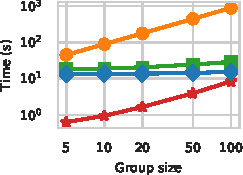
\includegraphics{./sources/plots/ged-walk/ged-time-vs-group.pdf}
\caption{Running time (s) of GED-Walk, GCC, GHC, and GBC maximization (note that $k$ is
in log-scale).}
\label{fig:ged-walk:scal-wrt-k}
\end{subfigure}\hfill
\begin{subfigure}[t]{.45\textwidth}
\centering
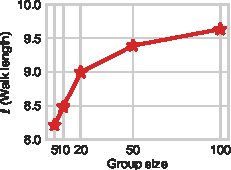
\includegraphics{./sources/plots/ged-walk/scalability-walk-length.pdf}
\caption{Length of the walks considered by our algorithm for GED-Walk maximization.}
\label{fig:ged-walk:scal-ell}
\end{subfigure}\hfill

\caption{Scalability \wrt group size of GED-Walk, GCC, GHC, and GBC maximization
(\Cref{fig:ged-walk:scal-wrt-k}), and highest walk length considered by our
GED-Walk maximization algorithm (\Cref{fig:ged-walk:scal-ell}).}
\label{fig:ged-walk:scalability-k-ell}
\end{figure}

\Cref{fig:ged-walk:scalability-k-ell} shows the average running time in seconds
of GED-Walk (GED), group-closeness (GCC), group-harmonic (GHC), and
group-betweenness (GBC) maximization for group sizes from 5 to 100 -- detailed
running times are reported in \Cref{tab:ged-walk:running-times},
\Cref{sec:ged-walk:running-times}. For small group sizes, GED-Walk can be
maximized much faster than the other considered measures: for $k = 5$, our
algorithm for GED-Walk maximization is on average \gedSpeedupGCCkfive,
\gedSpeedupGHCkfive, and \gedSpeedupGBCkfive faster than GCC, GHC and GBC maximization,
respectively, whereas for $k = 100$ it is respectively
\gedSpeedupGCCkHundred, \gedSpeedupGHCkhundred, and
\gedSpeedupGBCkHundred faster.
%
On the other hand, GCC and GHC maximization scale better than both GBC and GED-Walk
maximization \wrt the group size. This behavior is expected since the
evaluation of the marginal gain becomes computationally cheaper for GCC and GHC
for larger groups. This property, however, does
not apply to our algorithm for maximizing GED-Walk which, in turn, needs to increase
the length $\ell$ of the while the group grows -- see \Cref{algo:ged-lazy-greedy},
\Cref{line:ged-greedy:inc-l}.

Yet, one can also observe that the group-closeness score increases only very slowly
-- or more slowly than GED-Walk's -- when increasing the group size (see
\Cref{fig:ged-walk:large-groups-scores}). This means that, from a certain group
size on, the choice of a new group member hardly makes a difference for
group-closeness -- in most cases, only the distance to very close vertices can
be reduced. In that sense, GED-Walk seems to distinguish better between more
and less promising candidates.

\Cref{fig:ged-walk:scalability-k-ell} shows the length $\ell$ of the walks
considered by our algorithm \wrt the group size. In accordance to our
expectations about number of evaluations of $L_{\ell}(u)$ and $U_{\ell}(u)$ we
stated in \Cref{sec:ged-walk:maximizing-ged}, $\ell$ grows sub-linearly
\wrt $k$.

\subsection{Scalability to Large (Synthetic) Graphs}
%
\begin{figure}[tb]
\centering
\begin{subfigure}[t]{.24\textwidth}
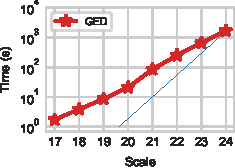
\includegraphics[width=\textwidth]{./sources/plots/ged-walk/ER_scalability.pdf}
\caption{\erdosr}
\label{fig:ged-walk:ER-scalability}
\end{subfigure}\hfill
\begin{subfigure}[t]{.24\textwidth}
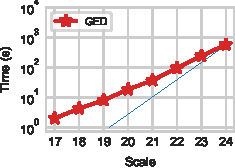
\includegraphics[width=\textwidth]{./sources/plots/ged-walk/RMAT_scalability.pdf}
\caption{R-MAT}
\label{fig:ged-walk:RMAT-scalability}
\end{subfigure}\hfill
\begin{subfigure}[t]{.24\textwidth}
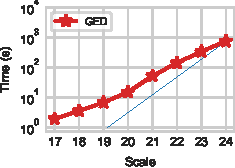
\includegraphics[width=\textwidth]{./sources/plots/ged-walk/BA_scalability.pdf}
\caption{Barab\`asi-Albert}
\label{fig:ged-walk:BA-scalability}
\end{subfigure}\hfill
\begin{subfigure}[t]{.24\textwidth}
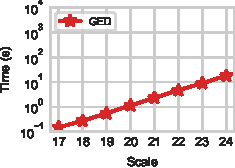
\includegraphics[width=\textwidth]{./sources/plots/ged-walk/RH_scalability.pdf}
\caption{Random hyperbolic}
\label{fig:ged-walk:RH-scalability}
\end{subfigure}
\caption{Running time (s) on 36 cores of our lazy greedy algorithm for GED-Walk
maximization on synthetic networks with $2^{17}$ to $2^{24}$ vertices, $k = 10$.
Data points are aggregated over three different randomly generated networks using
the geometric mean.}
\label{fig:ged-walk:synthetic-scalability}
\end{figure}

\begin{table}[tb]
\centering\footnotesize
\captionabove{Running time (s) of GED-Walk maximization on 36 cores on large
real-world networks, $k = 10$.}
\label{tab:ged-walk:time-large-insts}
\centering
\begin{tabular}{lrrrr}
\toprule
Network & Category & $n$ & $m$ & Time (s) \\
\midrule
petster-friendships-cat & Social & \numprint{148826} & \numprint{5447464} & \numprint{4.7}\\
dimacs9-W & Road & \numprint{6262104} & \numprint{7559642} & \numprint{45.3}\\
dimacs9-CTR & Road & \numprint{14081816} & \numprint{16933413} & \numprint{86.9}\\
flickr-growth & Social & \numprint{2173370} & \numprint{22729227} & \numprint{47.2}\\
soc-LiveJournal1 & Social & \numprint{4843953} & \numprint{42845684} & \numprint{35.0}\\
livejournal-links & Social & \numprint{5189808} & \numprint{48687945} & \numprint{47.1}\\
orkut-links & Social & \numprint{3072441} & \numprint{117184899} & \numprint{76.5}\\
dbpedia-link & Hyperlink & \numprint{18265512} & \numprint{126888089} & \numprint{348.7}\\
dimacs10-uk-2002 & Hyperlink & \numprint{18459128} & \numprint{261556721} & \numprint{47.5}\\
wikipedia\_link\_en & Hyperlink & \numprint{13591759} & \numprint{334590793} & \numprint{276.4}\\
\bottomrule
\end{tabular}

\end{table}

\Cref{fig:ged-walk:synthetic-scalability} shows the running time in seconds of
GED-Walk maximization with $k = 10$ on randomly generated networks using the
\erdosr, R-MAT, Barab\'asi-Albert, and random hyperbolic models models.
The thin blue lines represent the linear regression on the running times.
With respect to the running time curves, the regression lines either have a
steeper slope
(\Cref{fig:ged-walk:ER-scalability,fig:ged-walk:RMAT-scalability,fig:ged-walk:BA-scalability})
or, in the case of the random hyperbolic generator in
\Cref{fig:ged-walk:RH-scalability}, they match it almost perfectly. Thus, for
the network types and sizes under consideration, GED-Walk maximization scales
(empirically) linearly \wrt $n$.

\Cref{tab:ged-walk:time-large-insts} shows the running times in seconds of
GED-Walk maximization on large real-world instances with up to hundreds of
millions of edges with $k = 10$. For the largest networks, our algorithm needs
up to six minutes to finish, but in most cases it requires only around one
minute.

\subsection{Parallel Scalability}
%

\begin{figure}[tb]
\centering
\begin{subfigure}[t]{\textwidth}
\centering

\includegraphics{./sources/plots/ged-walk/legend-ged-time-vs-group.pdf}
\end{subfigure}\smallskip

\hfill
\begin{subfigure}[t]{.45\textwidth}
\centering
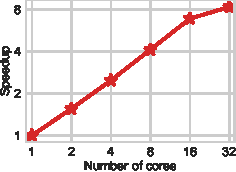
\includegraphics{./sources/plots/ged-walk/parallel-scalability.pdf}
\caption{Multi-core speedups of GED-Walk maximization over single-core GED-Walk
maximization.}
\label{fig:ged-walk:parallel-speedup}
\end{subfigure}\hfill
\begin{subfigure}[t]{.45\textwidth}
\centering
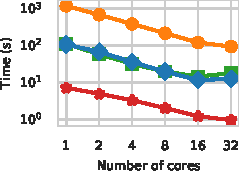
\includegraphics{./sources/plots/ged-walk/ged-multi-core-scal.pdf}
\caption{Running time of GED-Walk, GCC, GHC, and GBC maximization \wrt the number of
cores.}
\label{fig:ged-walk:parallel-time}
\end{subfigure}\hfill

\caption{Parallel scalability of GED-Walk, GCC, GHC, and GBC maximization, $k = 10$.
Data points are aggregated over the instances of \Cref{tab:ged-walk:real-world-insts}
using the geometric mean.}
\label{fig:ged-walk:parallel-scalability}
\end{figure}

As stated in \Cref{sec:ged-walk:compute-ged}, the algorithm to compute GED-Walk
can be parallelized easily by computing $\phit_i(u)$ and $\pmiss_i(u)$ in
parallel for different $u \in V$. \Cref{fig:ged-walk:parallel-speedup} shows
the parallel speedup of our algorithm for maximizing GED-Walk over itself
running on a single core for $k = 10$.
The scalability is moderate up to 16 cores, while on 32 cores it does not gain much
additional speedup. A similar behavior was observed before for
group-closeness~\cite{DBLP:conf/alenex/BergaminiGM18}. \Cref{fig:ged-walk:parallel-time}
shows the running time in seconds of GED-Walk, GBC, and GCC maximization with increasing
number of cores, for $k = 10$.
On a single core, GED-Walk maximization is on average
\gedAlgoSpeedupGCC, \gedAlgoSpeedupGHC, and \gedAlgoSpeedupGBC faster than GCC,
GHC, and GBC maximization, respectively.
As we increase the number of cores, the decrease of the running time of the
three algorithms is comparable -- except for GCC and GHC on 32 cores: In this
case, GCC and GHC are slower than on 16 cores on the considered instances.

The limited scalability affecting all three algorithms is probably due to memory
latency becoming a bottleneck in the execution on multiple
cores~\cite{DBLP:conf/icpp/BaderCF05,DBLP:journals/ppl/LumsdaineGHB07}.
Further, \Cref{fig:ged-walk:parallel-time} shows that, on 16 cores, our
algorithm for GED-Walk maximization finishes on average within a few seconds.
Here the running time of the algorithm is dominated by its sequential parts,
and it is not surprising that adding 16 more cores does not speed the algorithm
up substantially.

\subsection{Scalability with Large Groups}
%
\begin{figure}[tb]
\centering
\begin{subfigure}[t]{\textwidth}
\centering

\includegraphics{./sources/plots/ged-walk/legend-ged-time-vs-group-large.pdf}
\end{subfigure}\medskip

\hfill
\begin{subfigure}[t]{.45\textwidth}
\centering
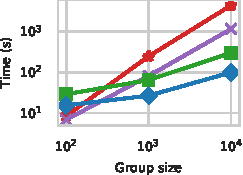
\includegraphics{./sources/plots/ged-walk/ged-time-vs-group-large.pdf}
\caption{Running time (s) of GED-Walk, GCC, and GHC maximization.}
\label{fig:ged-walk:large-groups-time}
\end{subfigure}\hfill
\begin{subfigure}[t]{.45\textwidth}
\centering
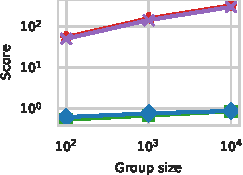
\includegraphics{./sources/plots/ged-walk/ged-score-vs-group-large.pdf}
\caption{GED-Walk, group-harmonic, and group-closeness scores of groups
computed by GED-Walk, GCC, and GHC maximization. For each $k$, scores are
divided by the scores for $k = 1$.}
\label{fig:ged-walk:large-groups-scores}
\end{subfigure}\hfill

\caption{Running time (s) and scores of GED-Walk with lazy greedy
(GED), and stochastic greedy (GED-S) strategies with large $k$ (log-scale).
Data points are aggregated over the instances of \Cref{tab:ged-walk:real-world-insts}
using the geometric mean.}
\end{figure}

We evaluate the performance of the stochastic algorithm with $\epsilon =
\numprint{0.5}$ and $\eta = \numprint{0.1}$ on large groups.
\Cref{fig:ged-walk:large-groups-time} shows the running time of GED-Walk
(both lazy and stochastic greedy strategies) GCC, and GHC maximization for
large values of $k$. For $k \ge \numprint{1000}$, the stochastic algorithm
is significantly faster than the lazy algorithm. However, as explained in
\Cref{sec:ged-walk:exp-scalability-k}, GCC maximization scales better
than both GED strategies \wrt $k$, and for $k \ge \numprint{1000}$ it is
even faster than GED-S.
%
On the other hand, \Cref{fig:ged-walk:large-groups-scores} shows the
relative GED-Walk, group-harmonic, and group-closeness scores of the groups
computed using GED, GED-S, GCC, and GHC maximization algorithms.
Results demonstrate that the stochastic greedy approach computes groups
with nearly the same quality as GED in less time, which makes it a
reasonable alternative to lazy greedy for large values of $k$.

\subsection{Impact of Parameter $\alpha$}
\label{sec:ged-walk:impact-of-alpha}
%
\begin{figure}[tb]
\centering

\begin{subfigure}[t]{.55\textwidth}
\centering
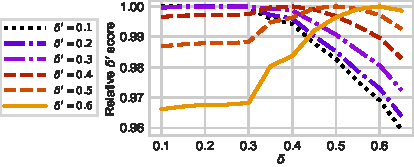
\includegraphics{./sources/plots/ged-walk/delta-relative-score.pdf}
\caption{Relative $\delta'$ score
(\ie $\ged^{\delta'}(S^{\delta}) / \ged^{\delta}(S^{\delta})$) for
$\delta,\delta' \in [\numprint{0.1}, \ldots, \numprint{0.6}]$,
$\epsilon = \numprint{0.1}$ and $k = 10$.}
\label{fig:ged-walk:delta-rel-score}
\end{subfigure}\hfill
\begin{subfigure}[t]{.4\textwidth}
\centering
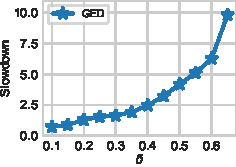
\includegraphics{./sources/plots/ged-walk/delta-run-time.pdf}
\caption{Slowdown of our algorithm for maximizing GED-Walk using
the spectral bound with $\alpha = \delta/\sigma_{\max}$ over
the lazy algorithm using the combinatorial bound.}
\label{fig:ged-walk:delta-slowdown}
\end{subfigure}\hfill

\caption{Quality and running time performance of our GED-Walk maximization
algorithm using the spectral bound. Data points are aggregated over the instances
of \Cref{tab:ged-walk:real-world-insts} using the geometric mean.}
\label{fig:ged-walk:alpha-impact}
\end{figure}

We now analyze how different settings of the parameter $\alpha$ impact the
groups computed by our algorithm for GED-Walk maximization. For this experiment
we use the spectral bound (see \Cref{eq:ged-walk:spectral-bound}).
\Cref{prop:ged-walk:convergence} implies that GED-Walk converges iff
$\alpha < 1/\sigma_{\max}$. Let $\delta \in (0, 1]$; obviously, GED-Walk also
converges if $\alpha < \delta / \sigma_{\max}$. In this experiment, we compute
groups $S^{\delta}$ for a certain value $\alpha = \delta/\sigma_{\max}$
and we measure of the resulting group using $\alpha' = \delta'/\sigma_{\max}$.
We denote this score by $\ged^{\delta'}(S^{\delta})$.

\Cref{fig:ged-walk:delta-rel-score} shows the ratio $\ged^{\delta'}(S^{\delta})
/ \ged^{\delta}(S^{\delta})$ with
$\delta, \delta' \in [\numprint{0.1}, \ldots, \numprint{0.6}]$, $\epsilon =
\numprint{0.1}$ and $k = 10$.
%
\Cref{fig:ged-walk:delta-slowdown} shows the slowdown, \ie running time of computing
$S^{\delta}$ divided by the running time of the lazy algorithm using the combinatorial
bound. Computing $\ged^{\delta'}(S^{\delta})$ with $\delta\in[\numprint{0.1}, \ldots,\numprint{0.3}]$
yields similar scores independently of $\delta$, meaning that the GED-Walk score of a group
does not change significantly within such an interval for $\delta$. Increasing $\delta$
above $\numprint{0.3}$, however, leads to a noticeable reduction of the relative
scores computed using $\delta' \le \numprint{0.3}$ and to a steeper growth of the ones
computed using $\delta' \ge \numprint{0.5}$.

\section{Applications of GED-Walk}
%
We demonstrate the relevance of GED-Walk for graph mining applications
by showing that it improves the performance of two popular graph mining tasks:
semi-supervised vertex classification and graph classification.
As a preprocessing step, for both tasks before applying GED-Walk we first construct a weighted
graph using the symmetrically normalized adjacency matrix $\Deg^{\frac 12}\Adj\Deg^{\frac 12}$,
which is often used in the literature~\cite{DBLP:conf/iclr/KipfW17,DBLP:conf/nips/ZhouBLWS03}.\footnote{
Recall that $\Deg$ is the degree matrix, see \Cref{sec:prelim-graphs}.}
Here, instead of taking the contribution of an $i$-walk $(e_1, \ldots, e_i)$ to be $\alpha$, we
define it to be $\alpha\prod_{j = 1}^i w(e_j)$, where $w(e_j) \le 1$ is the edge weight
of edge $e_j$. Except for the introduction of coefficients in the recurrences $\phit$ and
$\pmiss$, no modifications of our algorithms are required. Compared to our unweighted definition
of GED-Walk, this weighted variant converges even faster, as the contribution of each walk is
smaller.


\subsection{Vertex Classification}
\label{sec:ged-walk:vertex-class}
%
\begin{figure}[tb]

\hfill
\begin{subfigure}[t]{.45\textwidth}
\centering
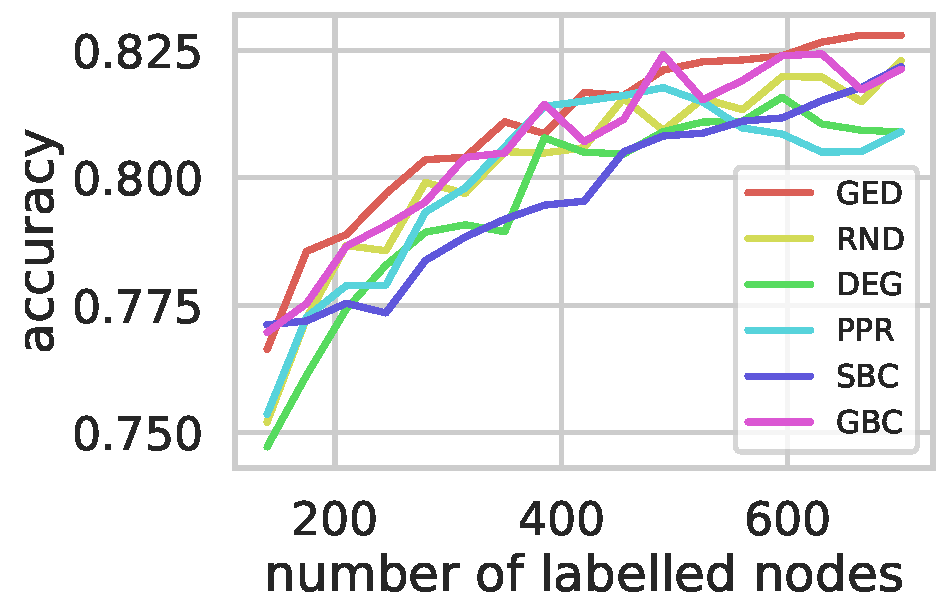
\includegraphics[width=.8\textwidth]{./sources/plots/ged-walk/node_classification_cora_ml.pdf}
\caption{Cora}
\end{subfigure}\hfill
\begin{subfigure}[t]{.45\textwidth}
\centering
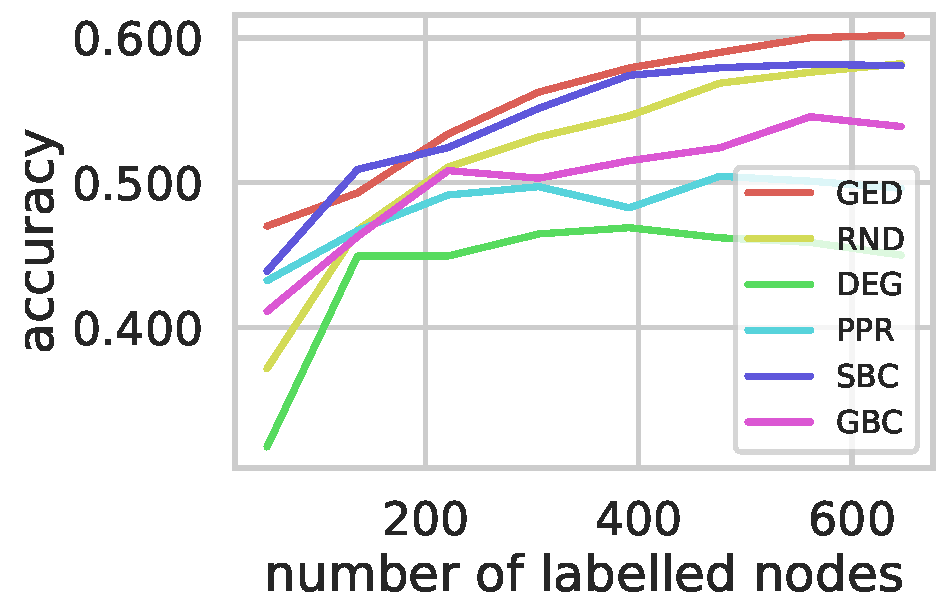
\includegraphics[width=.8\textwidth]{./sources/plots/ged-walk/node_classification_wiki.pdf}
\caption{Wiki}
\end{subfigure}\hfill

\caption{Semi-supervised vertex classification accuracy for different strategies
for choosing the training set.}
\label{fig:ged-walk:vertex-class}
\end{figure}

Vertex classification is a fundamental graph
mining problem where the goal is to predict the class labels of all vertices in
a graph given a small set of labelled vertices and the graph
structure~\cite{DBLP:journals/tnn/ChapelleSZ09}. The choice of which vertices
we label (\ie the vertices we include in the training set) before building a
classification model can have a significant impact on the test accuracy,
especially when the number of labelled vertices is small compared to the size
of the
graph~\cite{DBLP:conf/waw/AvrachenkovGS13,DBLP:journals/corr/abs-1811-05868}.
Since many models rely on diffusion to propagate information on the
graph~\cite{DBLP:journals/tnn/ChapelleSZ09}, we expect that selecting a
training set with high GED-Walk centrality will improve diffusion, and thus
also the model's accuracy. To test this hypothesis, we evaluate the performance
of Label Propagation~\cite{chapelle2009semi,DBLP:conf/nips/ZhouBLWS03} given
different strategies for choosing the training set.
The choice of the vertices for the training set can influence the
accuracy of the classifier, especially when the number of labelled
vertices is small compared to
$n$~\cite{DBLP:conf/waw/AvrachenkovGS13,DBLP:journals/corr/abs-1811-05868}.

A key aspect in semi-supervised learning problems is the so-called
\emph{cluster assumption}, \ie vertices that are close or that belong
to the same cluster typically have the same
label~\cite{DBLP:conf/nips/ChapelleWS02,DBLP:conf/nips/ZhouBLWS03}.
Several models label vertices by propagating information through
the graph via diffusion~\cite{DBLP:journals/tnn/ChapelleSZ09}.
We expect GED-Walk to cover the graph more thoroughly
than shortest-path based group centrality measures. Therefore, we conjecture
that choosing vertices with high GED-Walk improves the
diffusion -- and thus the accuracy of propagation-based models. We test this
hypothesis by comparing the classification accuracy of the label propagation
model~\cite{DBLP:journals/tnn/ChapelleSZ09,DBLP:conf/nips/ZhouBLWS03}
where the training set is chosen using different strategies.\footnote{While
this model is less powerful than state-of-the-art predictors,
our strategy to select the training set could also be applied to more
sophisticated models like graph neural networks.}
The main idea of label propagation is to start from a small number of
labelled vertices and each vertex iteratively propagates its label to
its neighbors until convergence.

In our experiments, we use the Normalized
Laplacian variant of the Label Propagation model as our baseline\footnote{Our
strategy to select the training set also applies to more sophisticated vertex
classification models such as graph neural
networks~\cite{DBLP:conf/iclr/KipfW17}.} and we set the value for the return
probability hyper-parameter to $\numprint{0.85}$.

We evaluate the classification accuracy on two common benchmark
graphs: Cora ($n = \numprint{2810}$, $m = \numprint{7981}$) and Wiki ($n = \numprint{2357}$,
$m = \numprint{11592}$)~\cite{sen2008collective}. We let the vertices with highest
GED-Walk centrality be in the training set and the rest of the vertices be in the
test set. We compare GED-Walk with the following baselines for selecting the
training set: RND (select vertices at random, with results averaged over 10 trials),
DEG (select the vertices with highest degree), SBC (select vertices with highest individual
betweenness centrality), GBC (select vertices with highest group-betweenness centrality),
and PPR (select vertices with highest Personalized PageRank).

\Cref{fig:ged-walk:vertex-class} shows that, for both the considered datasets and
across different number of labelled vertices, selecting the training set using GED-Walk
leads to highest (or comparable) test accuracy. Furthermore, while the second-best baseline
strategy is different on different datasets -- on Cora it is the GBC strategy while on
Wiki it is the SBC strategy), GED-Walk is consistently better.
Overall, these results confirm our hypothesis.

\subsection{Graph Classification}
%
\begin{table}[tb]
\centering
\footnotesize
\captionabove{Graph classification datasets.}
\label{tab:ged-walk:graph-class-data-sets}
\begin{tabular}{lrr}
\toprule
Dataset 							& \# of graphs & \# of classes\\
\midrule
Mutagenicity \cite{DBLP:conf/sspr/RiesenB08,kazius2005derivation}	& \numprint{4337}		& 2 		\\
PROTEINS \cite{dobson2003distinguishing,DBLP:conf/ismb/BorgwardtOSVSK05}	& \numprint{1113}		& 2			\\
ENZYMES	\cite{DBLP:conf/ismb/BorgwardtOSVSK05,DBLP:journals/nar/SchomburgCEGHHS04}	& 600		& 6			\\
IMDB-BINARY \cite{DBLP:conf/kdd/YanardagV15}		& \numprint{1000}		& 2			\\
REDDIT-BINARY \cite{DBLP:conf/kdd/YanardagV15} 	& \numprint{2000}		& 2			\\
\bottomrule
\end{tabular}


\end{table}

Graph classification is another fundamental graph mining problem. The goal is to
classify entire graphs based on features derived from their topology/structure.
In contrast to the vertex classification task where each dataset is a single
graph, here each dataset consists of many graphs with varying size and their
associated ground-truth class labels.
In this setting, our hypothesis is that groups of vertices with high
GED-Walk centrality capture rich information about the graph structure and thus
can be used to derive features that are useful for graph classification.

To extract features based on GED-Walk, we first compute the group of $k$ vertices
with highest (approximate) group centrality score. The group centrality score
is the first feature that we extract. In addition, we summarize the marginal gains
of all the remaining vertices in the graph in a histogram with $b$ bins.
We concatenate these features to get a feature vector $\vect{x}_i \in \real^{b + 1}$
for each graph $i$ in the dataset.
These features are useful since graphs with similar structure will have
similar group scores and marginal gains. We denote this base setting by \textsc{Ged}.

In addition, we obtain the topic-sensitive PageRank vector of each graph, where
we specify the teleport set to be equal to the vertices in the group with highest
(approximate) group centrality. Then, we summarize this vector (i) by using  a histogram
of $b$ bins and (ii) by extracting the top $p$ values, denoted by \textsc{PPR-H}
and \textsc{PPR-T}, respectively. Intuitively, these features capture the amount of diffusion
in the graph.

As a strong baseline, we compute the eigenvalues of the adjacency matrix and
summarize them (i) in a histogram of $b$ bins and (ii) by extracting the top $p$
eigenvalues, denoted by \textsc{Eig-H} and \textsc{Eig-T}, respectively.
This latter strategy is inspired by recent work on graph
classification~\cite{galland2019invariant} showing that spectral features can outperform
deep-learning based approaches. Further, the ability of efficiently compute the
eigenvalue histograms motivates using them as a feature for graph
classification~\cite{DBLP:conf/kdd/DongBB19}.
Similarly, a strong advantage of these features based on GED-Walk is that we can
efficiently compute them.
Last, we also combine the spectral- and GED-based features by concatenation, \ie
\textsc{Eig-T+GED} denotes the combination of \textsc{Eig-T} and \textsc{Ged}
features.
%
In the following experiments, we fix the value of the hyper-parameters $k = 10$,
$b = 20$, and $p = 10$; in practice, however, these parameters can also be tuned
using, for example, cross-validation. We split the data into $80\%$ training
and $20\%$ test set and average the results for 10 independent random splits.

\begin{table}[tb]
\centering
\footnotesize
\captionabove{Graph classification accuracy (in \%) on the datasets of
\Cref{tab:ged-walk:graph-class-data-sets}. Best performance per dataset marked
in bold.}
\label{tab:ged-walk:graph-class}
\begin{tabular}{lrrrrr}
\toprule
Dataset &  ENZ. &  IMD. &  Mut. &  PRO. &  RED. \\
\midrule
\textsc{Eig}-T                           &    23.02 &        56.59 &         56.90 &     73.35 &          75.31 \\
\textsc{Eig}-H                           &    23.47 &        70.28 &         68.88 &     72.42 &          72.02 \\ \midrule
\textsc{Ged}                             &    19.18 &        60.64 &         64.51 &     71.95 &          70.59 \\
\textsc{Ged+PPR}$^*$-H                   &    20.85 &        65.18 &         65.46 &     72.18 &          71.59 \\
\textsc{Ged+PPR}$^{**}$-H                &    20.39 &        66.27 &         65.86 &     72.44 &          75.95 \\\midrule
\textsc{Eig}-T+\textsc{Ged}-T            &    26.46 &        63.56 &         64.14 &\textbf{74.06} &      80.18 \\
\textsc{Eig}-H+\textsc{Ged}-H            &    23.14 &        69.74 &         69.08 &     73.13 &          75.16 \\\midrule
\textsc{Eig}-T+ & \multirow{2}{*}{27.45} & \multirow{2}{*}{69.25} & \multirow{2}{*}{62.78} &\multirow{2}{*}{73.54} &\multirow{2}{*}{76.70}\\
\textsc{Ged+PPR}$^*$-T\\
\addlinespace[3pt]
\textsc{Eig}-H+    &\multirow{2}{*}{24.12} &\multirow{2}{*}{\textbf{71.62}}&\multirow{2}{*}{\textbf{69.18}}& \multirow{2}{*}{73.10} &\multirow{2}{*}{74.17} \\
\textsc{Ged+PPR}$^*$-H\\
\addlinespace[3pt]
\textsc{Eig}-T+ &\multirow{2}{*}{\textbf{27.88}} &\multirow{2}{*}{68.53} &\multirow{2}{*}{62.43} &\multirow{2}{*}{73.72}&\multirow{2}{*}{80.48} \\
\textsc{Ged+PPR}$^{**}$-T\\
\addlinespace[3pt]
\textsc{Eig}-H+ &\multirow{2}{*}{24.78}&\multirow{2}{*}{70.54}&\multirow{2}{*}{68.81}&\multirow{2}{*}{72.97}&\multirow{2}{*}{\textbf{81.43}}\\
\textsc{Ged+PPR}$^{**}$-H\\
\bottomrule
\multicolumn{6}{l}{$^*$: PageRank teleport probability 0.85;}\\
\multicolumn{6}{l}{$^{**}$: PageRank teleport probability 0.15}
\end{tabular}

\end{table}

\Cref{tab:ged-walk:graph-class} summarizes graph classification results over the instances
of \Cref{tab:ged-walk:graph-class-data-sets}.
Notice that enriching the baseline features with our GED-Walk-based features
improves the classification accuracy on all datasets, with variants
using all available features (\ie \textsc{Eig+Ged+PPR}) performing
best. Moreover, as shown in \Cref{tab:ged-walk:graph-class-acc}, using the most
central group according to GED-Walk as teleport set yields performance improvements
over standard PageRank -- \ie with teleport to all vertices.

In summary, these results show that GED-Walk captures meaningful information about
the graph structure that is complementary to baseline spectral features. We argue that
GED-Walk can be used as a relatively inexpensive to compute additional source of
information to enhance existing graph classification models.

\begin{table}[tb]
\centering
\setlength{\tabcolsep}{4pt}
\footnotesize
\captionabove{Graph classification accuracy (in \%) on the datasets of
\Cref{tab:ged-walk:graph-class-data-sets}. \textsc{PR} denotes PageRank with
all vertices as the teleport set.}
\label{tab:ged-walk:graph-class-acc}
\begin{tabular}{lrrrrr}
\toprule
Dataset &  ENZYMES &  IMDB-BINARY &  Mutagenicity &  PROTEINS &  REDDIT-BINARY \\
                                         &          &              &               &           &                \\
\midrule
\textsc{Eig}-H+\textsc{Ged+PPR}$^*$-H    &    24.12 &\textbf{71.62}& \textbf{69.18}&     73.10 &          74.17 \\
\textsc{Eig}-T+\textsc{Ged+PPR}$^*$-T    &    27.45 &        69.25 &         62.78 &     73.54 &          76.70 \\
\textsc{Eig}-H+\textsc{Ged+PPR}$^{**}$-H &    24.78 &        70.54 &         68.81 &     72.97 &  \textbf{81.43} \\
\textsc{Eig}-T+\textsc{Ged+PPR}$^{**}$-T &\textbf{27.88} &   68.53 &         62.43 &     73.72 &          80.48 \\
\textsc{Eig}-H+\textsc{Ged}              &    23.14 &        69.74 &         69.08 &     73.13 &          75.16 \\
\textsc{Eig}-T+\textsc{Ged}              &    26.46 &        63.56 &         64.14 &\textbf{74.06} &      80.18 \\
\textsc{Eig}-H+\textsc{PPR}$^*$-H        &    24.20 &\textbf{71.62}& \textbf{69.18}&     73.08 &          74.17 \\
\textsc{Eig}-T+\textsc{PPR}$^*$-T        &    27.49 &        69.25 &         62.78 &     73.56 &          76.71 \\
\textsc{Eig}-H+\textsc{PPR}$^{**}$-H     &    24.78 &        70.54 &         68.80 &     72.97 &  \textbf{81.43} \\
\textsc{Eig}-T+\textsc{PPR}$^{**}$-T     &\textbf{27.88} &   68.53 &         62.43 &     73.72 &          80.48 \\
\textsc{Eig}-H+\textsc{PR}$^*$-H         &    23.54 &        70.00 &         68.85 &     72.33 &          75.11 \\
\textsc{Eig}-T+\textsc{PR}$^*$-T         &    23.18 &        57.06 &         57.38 &     73.25 &          76.00 \\
\textsc{Eig}-H+\textsc{PR}$^{**}$-H      &    23.54 &        70.42 &         69.17 &     72.49 &          76.33 \\
\textsc{Eig}-T+\textsc{PR}$^{**}$-T      &    23.18 &        58.42 &         57.79 &     73.31 &          76.59 \\
\textsc{Eig}-H                           &    23.47 &        70.28 &         68.88 &     72.42 &          72.02 \\
\textsc{Eig}-T                           &    23.02 &        56.59 &         56.90 &     73.35 &          75.31 \\
\textsc{Ged+PPR}$^*$-H                   &    20.85 &        65.18 &         65.46 &     72.18 &          71.59 \\
\textsc{Ged+PPR}$^{**}$-H                &    20.39 &        66.27 &         65.86 &     72.44 &          75.95 \\
\textsc{Ged}                             &    19.18 &        60.64 &         64.51 &     71.95 &          70.59 \\
\textsc{PPR}$^*$-H                       &    21.01 &        60.93 &         60.44 &     71.79 &          72.74 \\
\textsc{PPR}$^{**}$-H                    &    19.46 &        66.39 &         62.27 &     71.86 &          73.79 \\
\textsc{PR}$^*$-H                        &    20.11 &        57.04 &         61.31 &     71.78 &          73.19 \\
\textsc{PR}$^*$-T                      &    16.98 &        51.15 &         55.85 &     71.84 &          69.66 \\
\textsc{PR}$^{**}$-H                     &    20.11 &        60.84 &         61.75 &     71.77 &          73.43 \\
\textsc{PR}$^{**}$-T                   &    16.98 &        56.64 &         57.19 &     72.12 &          73.31 \\
\bottomrule
\multicolumn{6}{l}{$^*$: PageRank teleport probability 0.85; $^{**}$: PageRank teleport probability 0.15}
\end{tabular}

\end{table}

\section{Experiments -- Group Forest Closeness}
%
As we did for GED-Walk, to demonstrate the relevance of group forest closeness
in graph mining applications, we apply it to semi-supervised vertex
classification~\cite{DBLP:journals/tnn/ChapelleSZ09} (see
\Cref{sec:ged-walk:vertex-class}).

\paragraph{Settings}
We implement our algorithm for forest closeness maximization
in C++ upon the NetworKit~\cite{DBLP:journals/netsci/StaudtSM16} toolkit and we
manage our experiments with
SimexPal~\cite{DBLP:journals/algorithms/AngrimanGLMNPT19} to ensure
reproducibility.

In our experiments, we used the Normalized Laplacian variant of label
propagation~\cite{DBLP:conf/nips/ZhouBLWS03}. We set the return probability
hyper-parameter to \numprint{0.85} and we evaluate its accuracy on two
well-known disconnected graph datasets: Cora ($n = \numprint{2708}$,
$m = \numprint{5278}$) and Citeseer ($n = \numprint{3264}$,
$m = \numprint{4536}$)~\cite{sen2008collective}.
Since this variant of label propagation cannot handle graphs with isolated
vertices (\ie zero-degree vertices), we remove all isolated vertices from
these datasets. For a fixed size $k$ of the training set, we select its
vertices as the group of vertices computed by our greedy algorithm for
group forest maximization and as the top-$k$ vertices with highest
estimated forest closeness. We also include several well-known
(individual) vertex selection strategies for comparison: average
over 10 random trials, the top-$k$ vertices with highest degree,
the top-$k$ vertices with highest betweenness centrality, and the
top-$k$ vertices with highest Personalized PageRank.

\begin{figure}[tb]
\centering
\begin{subfigure}[t]{\textwidth}
\centering
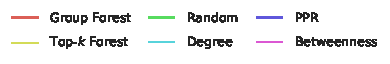
\includegraphics{sources/plots/el-clos/legend-node-class.pdf}
\end{subfigure}\smallskip

\begin{subfigure}[t]{.45\textwidth}
\centering
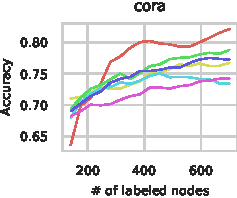
\includegraphics[width=.7\textwidth]{sources/plots/el-clos/node-class-cora.pdf}
\end{subfigure}\hfill
\begin{subfigure}[t]{.45\textwidth}
\centering
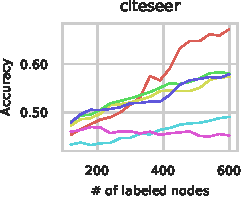
\includegraphics[width=.7\textwidth]{sources/plots/el-clos/node-class-citeseer.pdf}
\end{subfigure}
\caption{Accuracy in semi-supervised vertex classification in disconnected
graphs when using different strategies to create the training set.}
\label{fig:el-clos:vertex-class}
\end{figure}

\begin{figure}[tb]
\centering
\begin{subfigure}[t]{\textwidth}
\centering
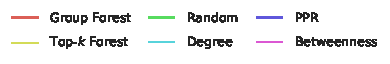
\includegraphics{sources/plots/el-clos/legend-node-class.pdf}
\end{subfigure}\smallskip

\begin{subfigure}[t]{.45\textwidth}
\centering
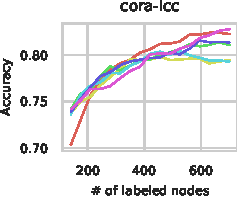
\includegraphics[width=.7\textwidth]{sources/plots/el-clos/node-class-cora_lcc.pdf}
\end{subfigure}\hfill
\begin{subfigure}[t]{.45\textwidth}
\centering
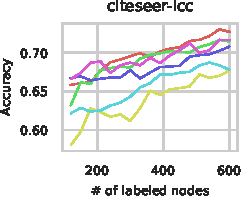
\includegraphics[width=.7\textwidth]{sources/plots/el-clos/node-class-citeseer_lcc.pdf}
\end{subfigure}
\caption{Accuracy in semi-supervised vertex classification on the largest
connected component of the datasets (Cora-lcc: $n = \numprint{2485}$,
$m = \numprint{5069}$; Citeseer-lcc: $n = \numprint{2110}$, $m = \numprint{3668}$)
when using different strategies to create the training set.}
\label{fig:el-clos:vertex-class-lcc}
\end{figure}

\paragraph{Results}
%
\Cref{fig:el-clos:vertex-class} shows that, for disconnected graphs
and for a moderate number of labelled vertices, selecting the training
set by group forest closeness maximization yields consistently
superior accuracy than strategies based on existing centrality measures
-- including top-$k$ forest farness.
As expected, the accuracy of existing measures improves if one considers
connected graphs. \Cref{fig:el-clos:vertex-class-lcc} shows the accuracy
for connected graphs when using different strategies to create the  training set.
Compared to disconnected graphs, the competitors perform better in this setting.
However, in our datasets, choosing the training set by group forest
maximization yields nearly the same accuracy as the best competitors.
The running time of our greedy algorithm for group forest maximization
is reported in \Cref{tab:el-clos:time-group-forest},
\Cref{apx:el-clos:group-forest-time}.

\section{Conclusions}
%
In this chapter, we addressed the issues of scaling group centrality
to large networks and the lack of electrical group centrality measures capable
of handling disconnected graphs.
We introduced two new centrality measures, GED-Walk and group forest closeness.
For the former, we implemented efficient
approximation algorithms for its maximization and for computing the GED-Walk
score of a given group.
For the latter, we adapted the cubic approximation algorithm from
Li \etal~\cite{DBLP:conf/www/0002PSYZ19}.

GED-Walk's descriptive power is demonstrated by
experiments on two fundamental graph mining tasks: both semi-supervised vertex
classification and graph classification benefit from the new measure. As
GED-Walk can be optimized faster than earlier group centrality measures, it is
often a viable replacement for more expensive measures in performance-sensitive
applications.
Group forest closeness achieved analogous results for the semi-supervised
vertex classification task on disconnected graphs.
On the other hand, cubic time cannot scale to large graphs; we leave the
development of faster approximation algorithms to maximize this measure
to future work.

In terms of running time, our algorithm for GED-Walk
maximization significantly outperforms the state-of-the-art algorithms for
maximizing group-closeness, group-harmonic, and group-betweenness centrality
when group sizes are at most 100. The fact that GED-Walk scales worse than
group-closeness and group-harmonic \wrt
to $k$ may seem as a limitation; however, we expect that many applications are
interested in group sizes considerably smaller than 100.

Experiments on synthetic networks indicate that our algorithm for GED-Walk
maximization scales linearly with the number of vertices.
For graphs with $2^{24}$ vertices and more than 100M edges, it needs up to
half an hour -- often less. In fact, our algorithm can maximize GED-Walk for
small groups on real-world graphs with hundreds of millions of edges within a
few minutes.
A promising direction for future research is to apply GED-Walk to other
practical applications. Examples include network and traffic
monitoring~\cite{DBLP:journals/ipl/DolevEPZ09,DBLP:journals/jits/PuzisAEBSP13},
the development of immunization strategies to lower the vulnerability of a
network to epidemic outbreaks~\cite{pastor2002immunization}, and improving
landmark-based shortest path queries~\cite{DBLP:conf/soda/GoldbergH05}.
